
\section{Plotting}
\label{sec:plotting}

% -----------------------------------------------------------------------

\begin{frame}
  \frametitle{Plotting}

  \begin{itemize}
  \item When saving plots, remember that the slides have a 4$\times$3
    aspect ratio, and try to fill up the slide
  \end{itemize}
  
\end{frame}

% -----------------------------------------------------------------------

\begin{frame}
  \begin{figure}[htp!]
    \centering
    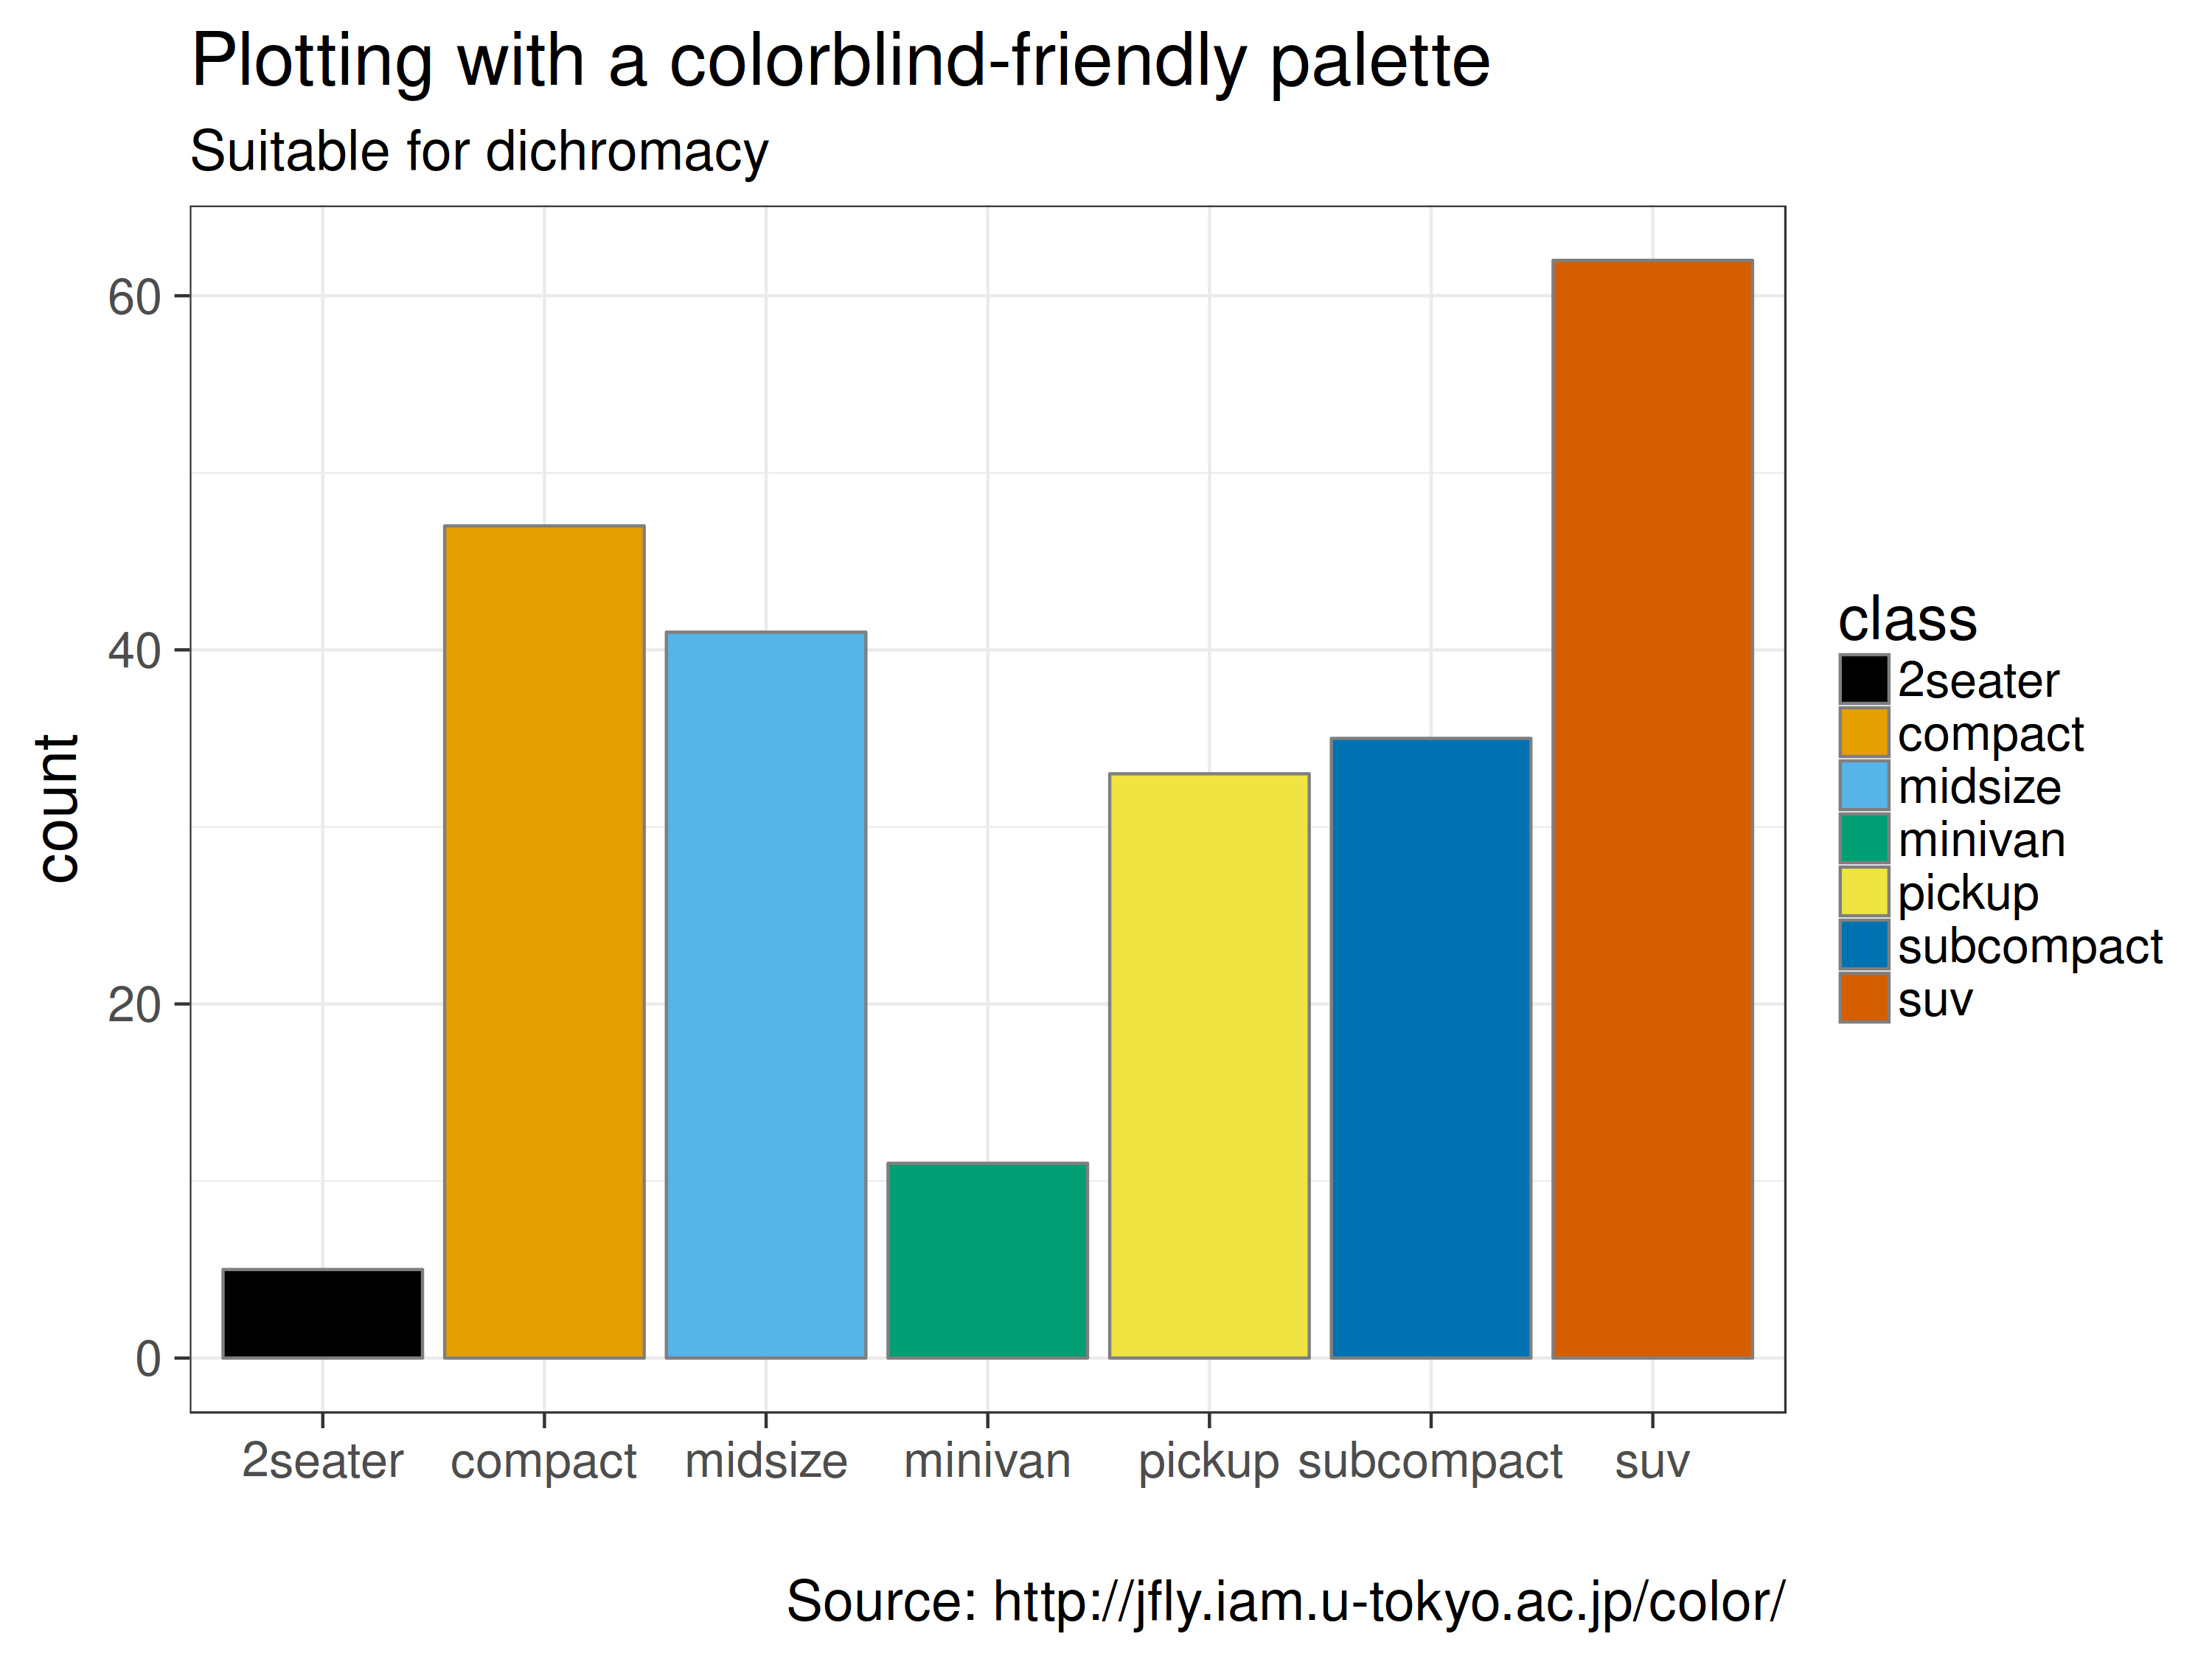
\includegraphics[width=0.9\linewidth]{fig/barchart-defaultfont.png}
  \end{figure}

  \small The default ggplot2 typeface is Helvetica, which looks OK
  except for the tight spacing between characters.
  
\end{frame}

% -----------------------------------------------------------------------

\begin{frame}
  \begin{figure}[htp!]
    \centering
    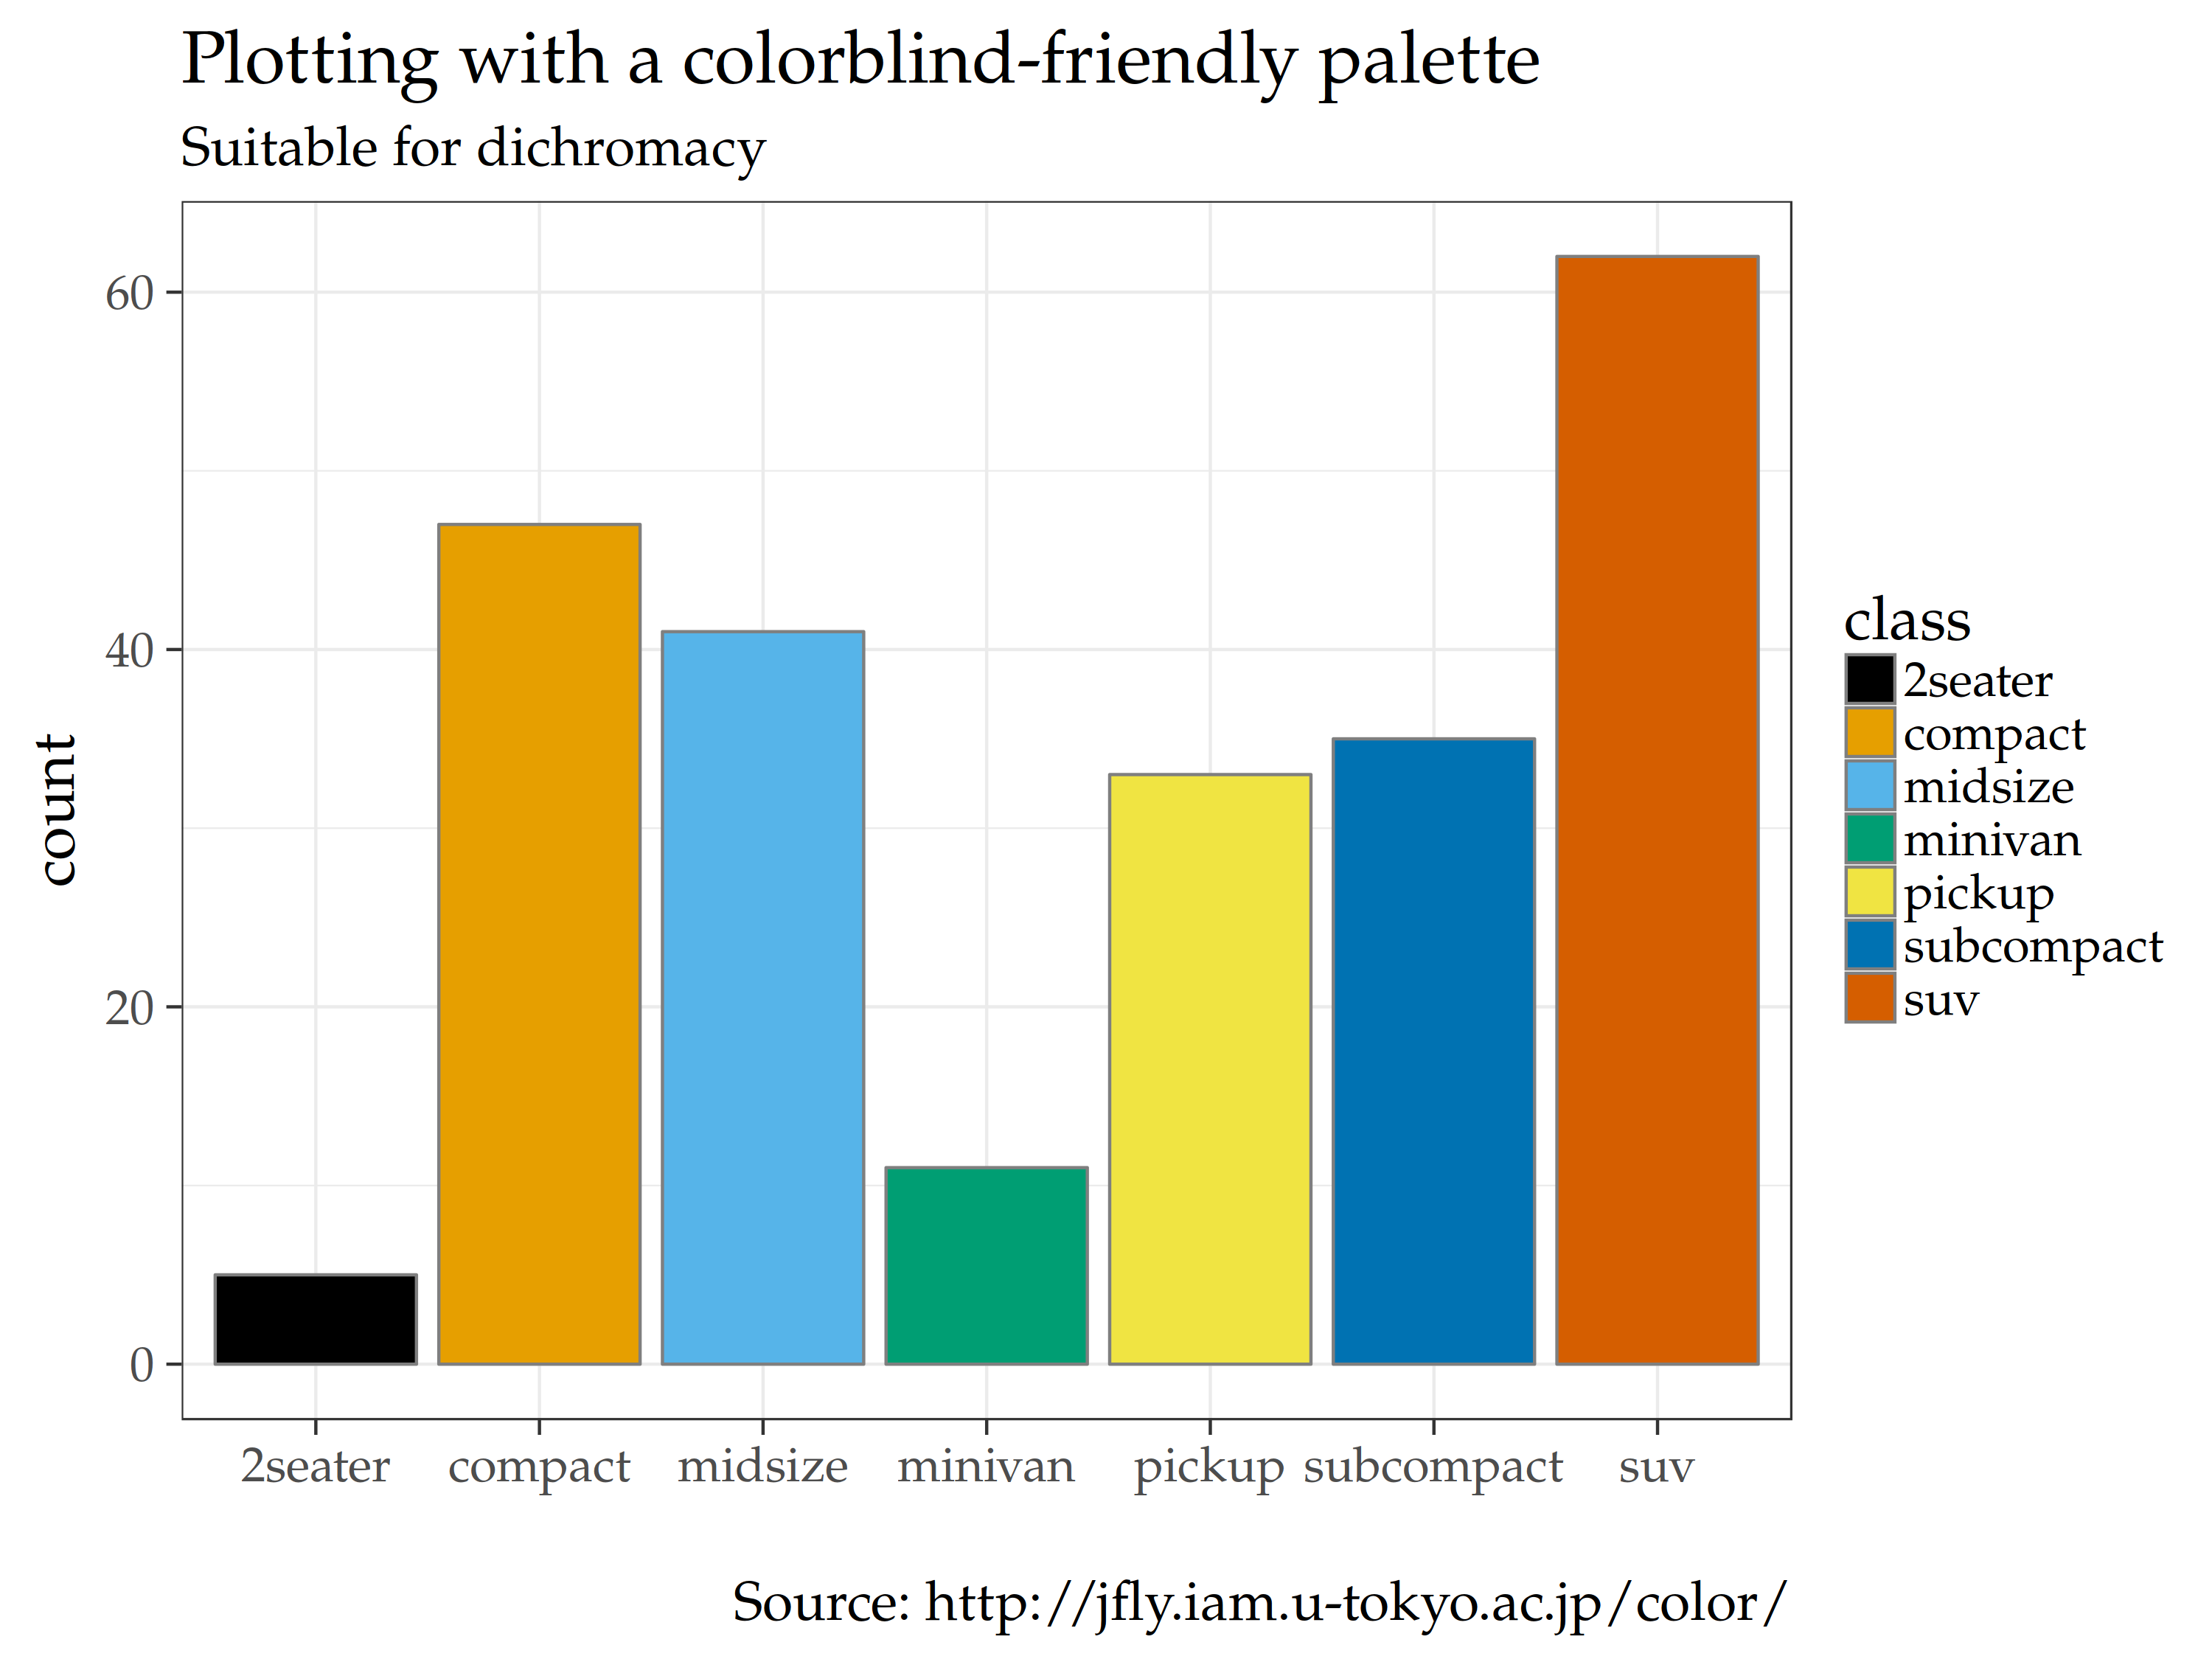
\includegraphics[width=0.9\linewidth]{fig/barchart-palatino.png}
  \end{figure}
  
  \small Palatino looks nice, but serifs are not optimal for
  legibility of text on a screen.
  
\end{frame}

% -----------------------------------------------------------------------

\begin{frame}
  \begin{figure}[htp!]
    \centering
    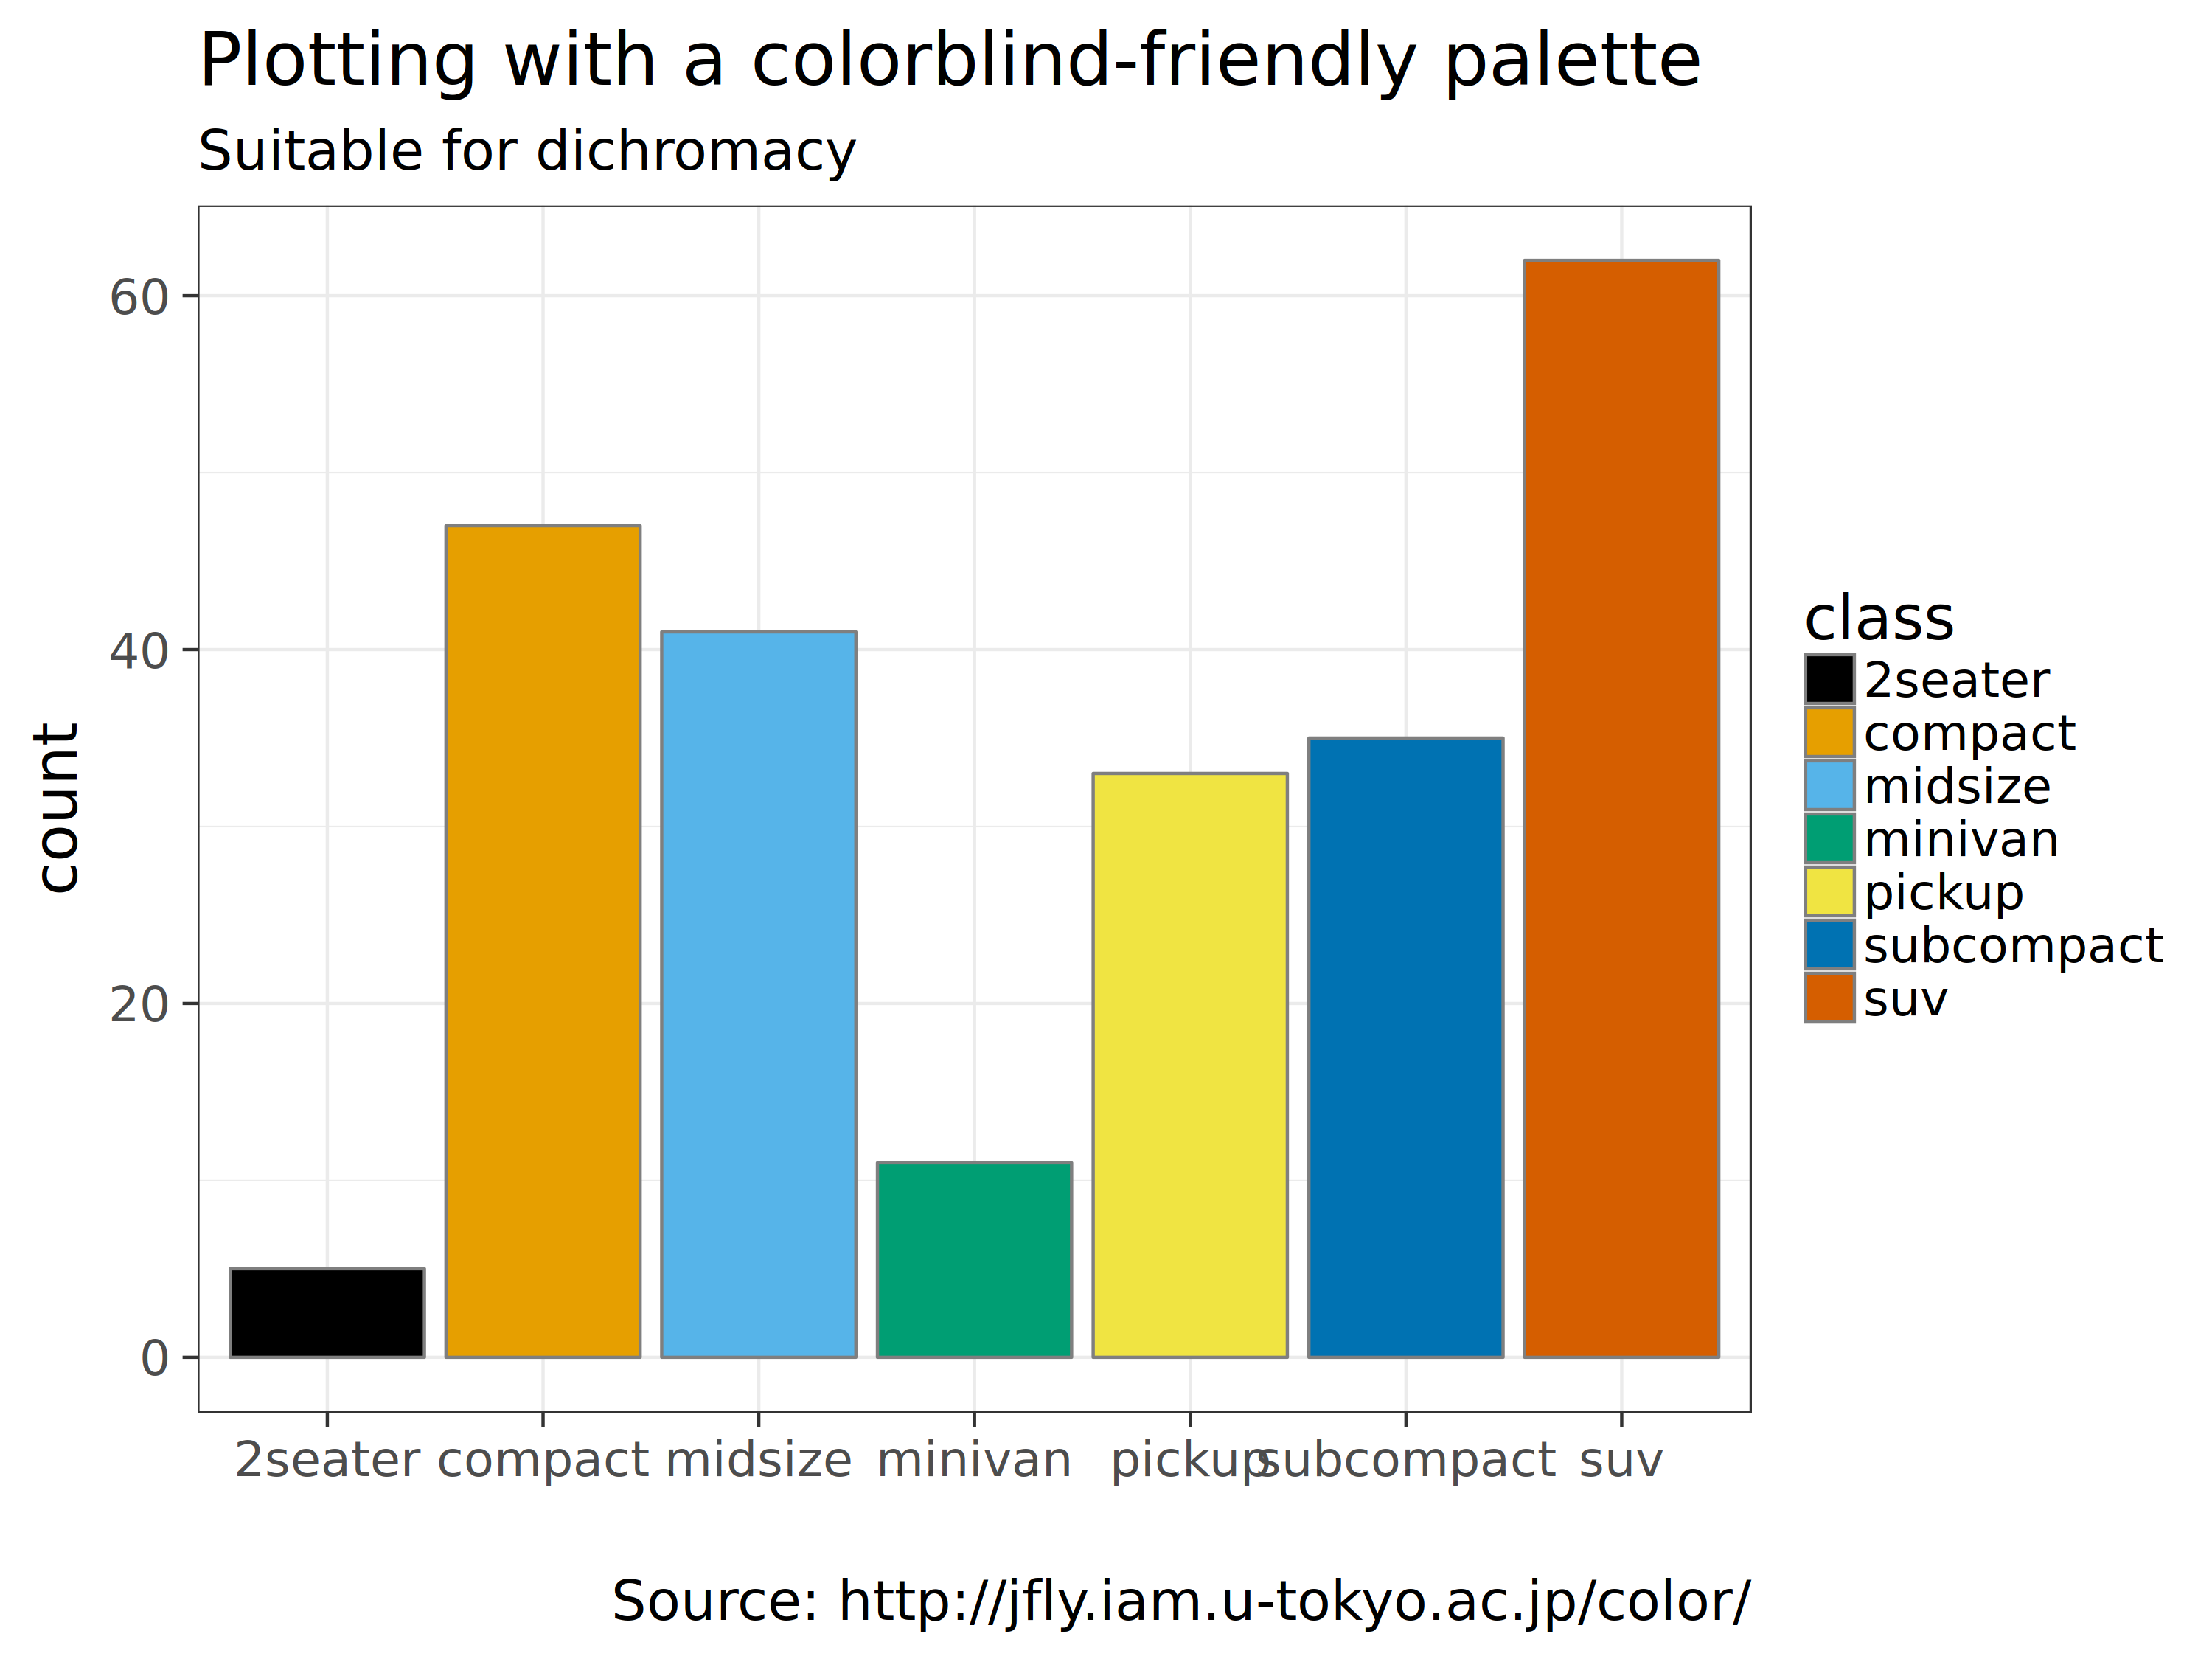
\includegraphics[width=0.9\linewidth]{fig/barchart-latosans.png}
  \end{figure}

  \small Lato Sans is like Helvetica, with more generous spacing.
  
\end{frame}

% -----------------------------------------------------------------------

\begin{frame}
  \begin{figure}[htp!]
    \centering
    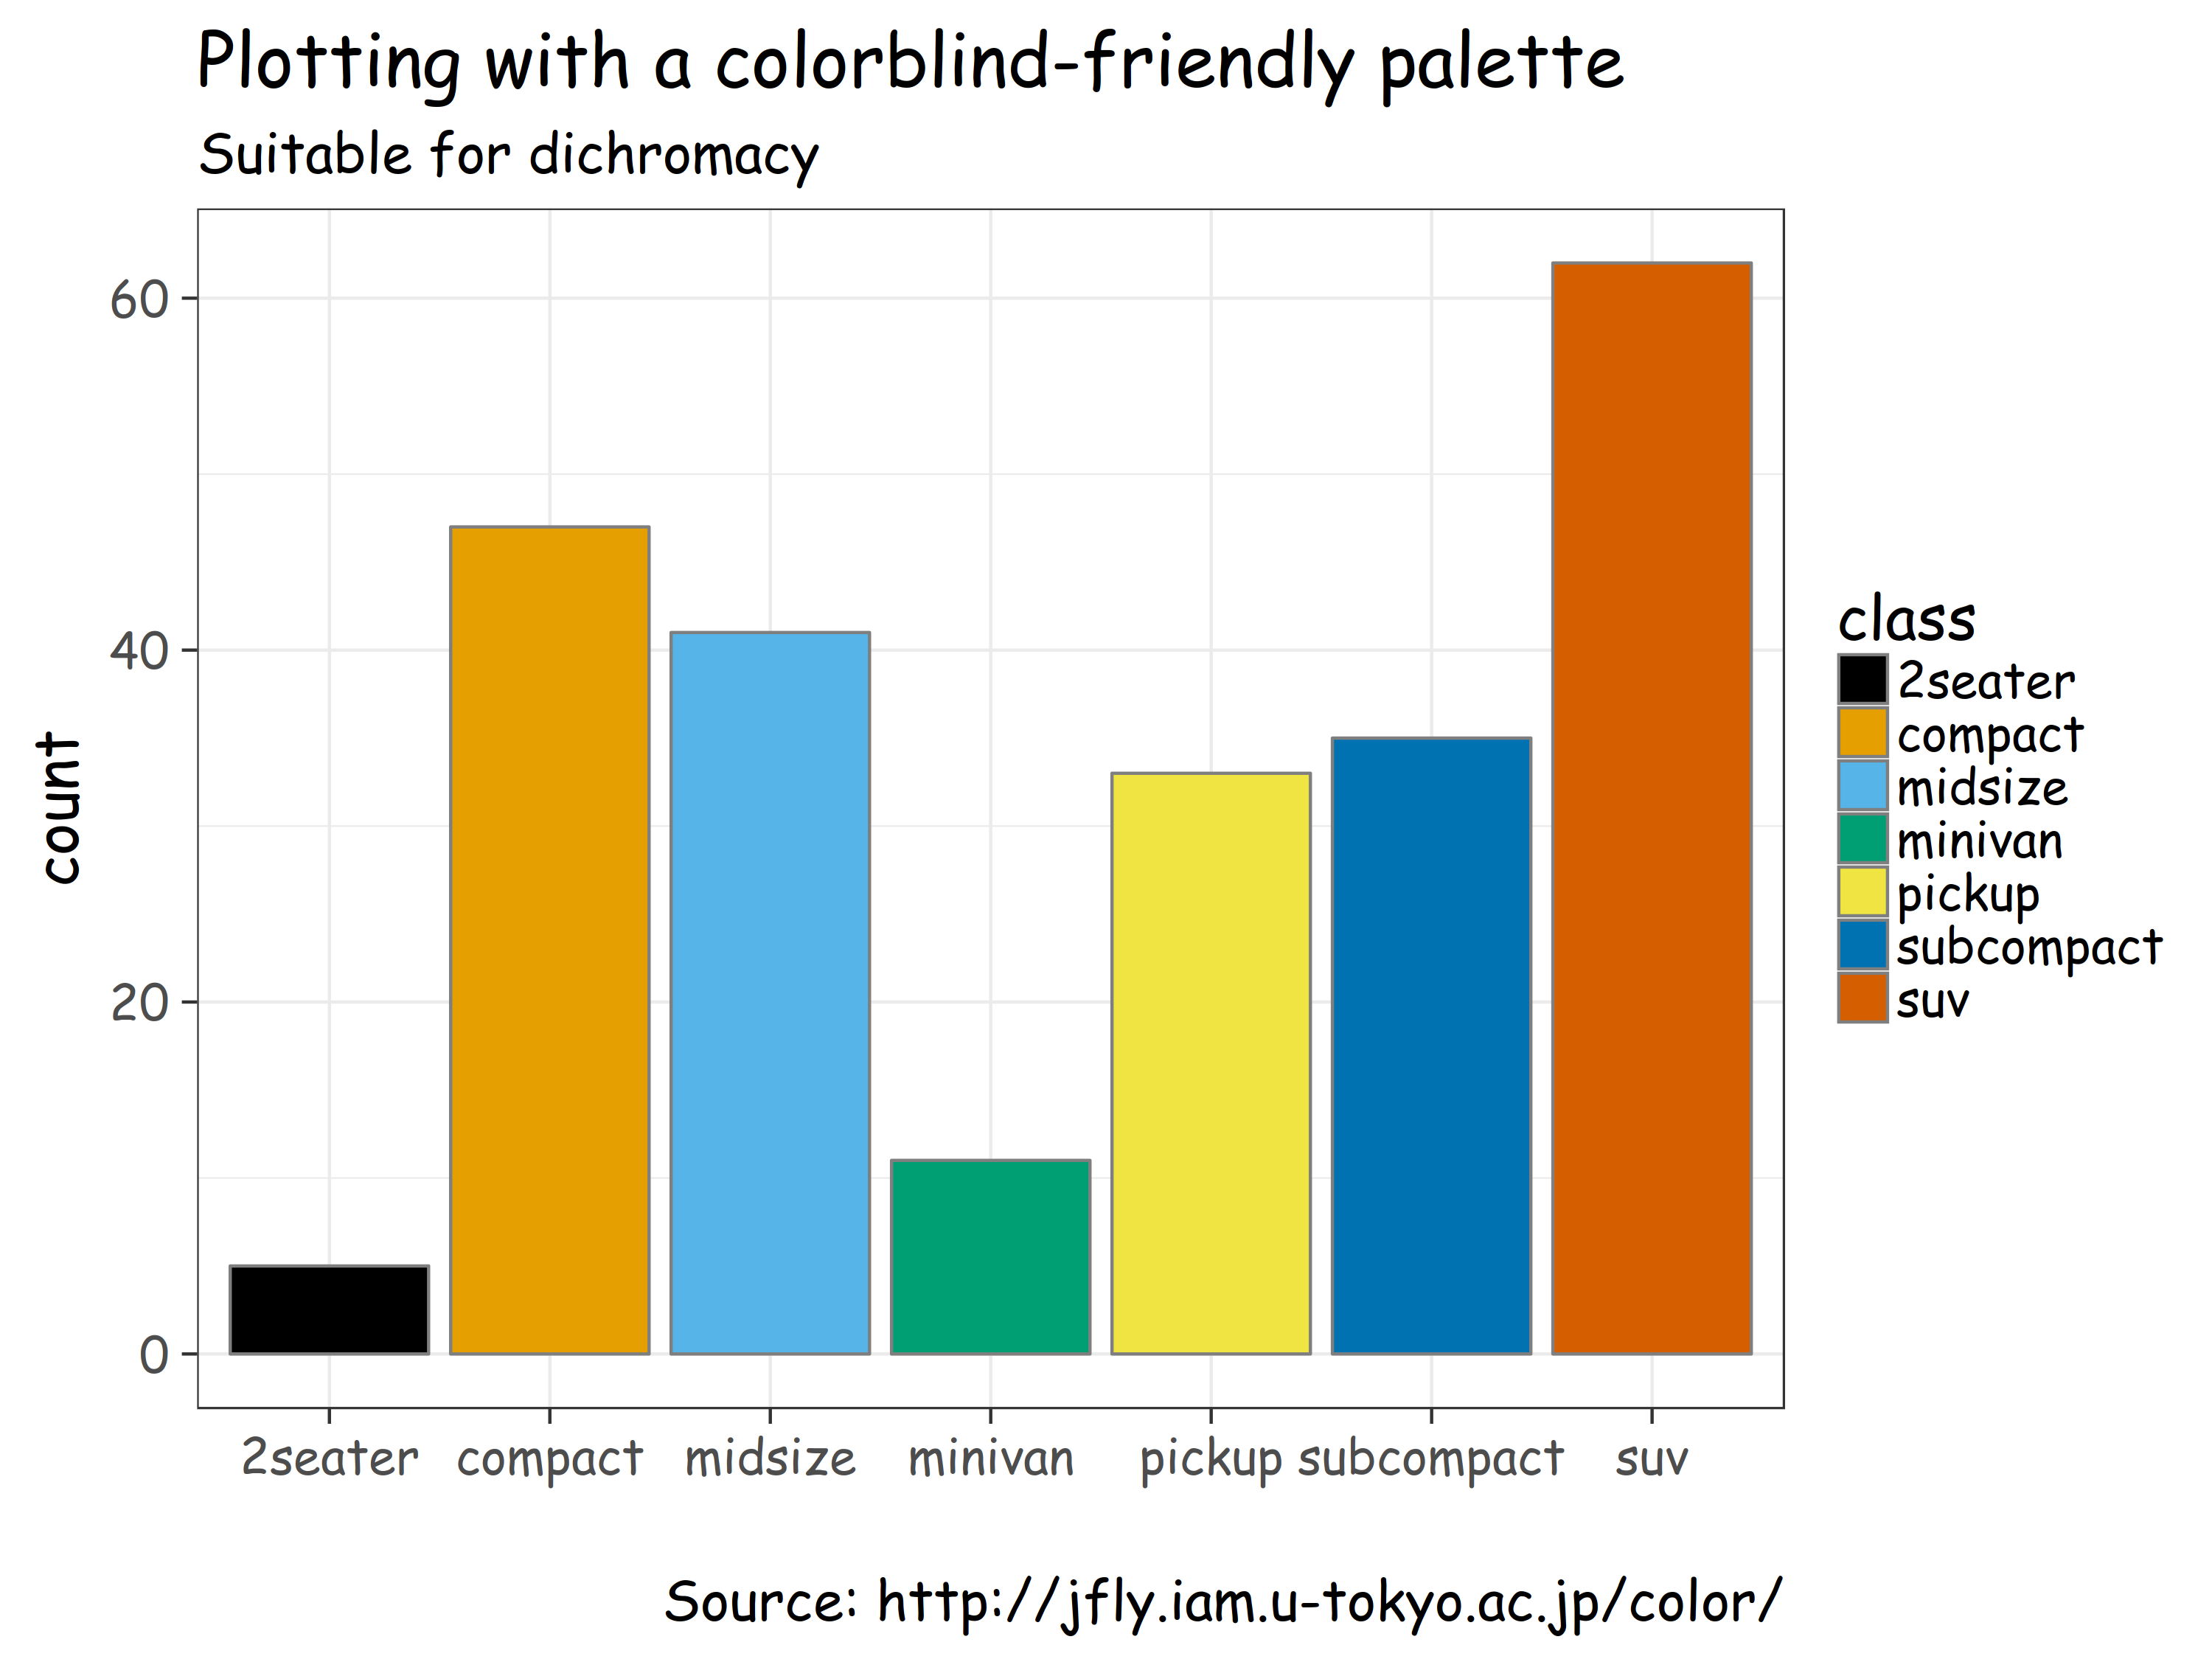
\includegraphics[width=0.9\linewidth]{fig/barchart-comicsansms.png}
  \end{figure}

  \small Comic Sans is hard to beat when it comes to legibility, and
  is also good for those with dyslexia.
  
\end{frame}

% -----------------------------------------------------------------------

%%% Local Variables:
%%% mode: latex
%%% TeX-master: "../main"
%%% End:
